\section{Scoreboard}

Imagine a scenario where a data structure maintains records of all instructions across functional units. 
Prior to the issue stage dispatching an instruction, several checks must be conducted:
\begin{enumerate}
    \item Availability of the required functional unit.
    \item Availability of input data, considering Read-After-Write (RAW) hazards.
    \item Safety in writing to the destination, taking into account Write-After-Read (WAR) and Write-After-Write (WAW) hazards.
    \item Detection of structural conflicts at the Write-Back (WB) stage.
\end{enumerate}

We introduce a data structure called the Correct Issues Table to keep track of the status of functional units. 
The fields are as follows:
\begin{table}[H]
    \centering
    \begin{tabular}{|c|c|cccc|}
        \hline
    \textbf{Name} & \textbf{Busy} & \textbf{Op} & \textbf{Dest} & \textbf{Src1} & \textbf{Src2} \\ \hline
    Int           &               &             &               &               &               \\
    Mem           &               &             &               &               &               \\ \hline
    Add1          &               &             &               &               &               \\
    Add2          &               &             &               &               &               \\
    Add3          &               &             &               &               &               \\ \hline
    Mult1         &               &             &               &               &               \\
    Mult2         &               &             &               &               &               \\ \hline
    Div           &               &             &               &               &               \\ \hline
    \end{tabular}
\end{table}
At the issue stage, the instruction $i$ consults this table using the following rules:
\begin{itemize}
    \item To check if the required functional unit is available, consult the busy column.
    \item For Read-After-Write (RAW) hazard detection, search the destination column for $i$'s sources.
    \item For Write-After-Read (WAR) hazard detection, search the source columns for $i$'s destination.
    \item For Write-After-Write (WAW) hazard detection, search the destination column for $i$'s destination.
\end{itemize}
An entry is added to the table if no hazard is detected. 
An entry is removed from the table after the Write-Back stage.

\paragraph*{Dynamic scheduling idea}
In the context of computer architecture and pipelined execution, dynamic scheduling addresses the issue of hardware stalls caused by data dependencies that cannot be resolved through bypassing or forwarding mechanisms.

Instead of letting instructions stall the pipeline, dynamic scheduling allows the hardware to rearrange the execution order of instructions dynamically. 
This enables instructions that are not dependent on stalled instructions to proceed, thus reducing pipeline stalls and improving overall performance.

Dynamic scheduling facilitates out-of-order execution, where instructions are executed as soon as their operands are available, regardless of their original order in the program. However, it also introduces the need to handle hazards such as Write-After-Read (WAR) and Write-After-Write (WAW) data hazards, which may arise due to the out-of-order execution.

The concept of dynamic scheduling was first implemented in the CDC6600 supercomputer in 1963, marking a significant advancement in computer architecture by allowing for more efficient utilization of hardware resources and better performance in pipelined execution.

\subsection{CDC6600 scoreboard}
The CDC6600 Scoreboard is designed to manage instruction execution efficiently while ensuring data dependencies are handled properly. Here's a revised version of its key features:
\begin{itemize}
    \item Instructions are dispatched in sequential order to functional units, as long as there are no structural hazards or Write-After-Write (WAW) hazards.
    \item If a structural hazard occurs or no functional units are available, the execution is stalled.
    \item Each register has only one pending write operation at a time.
    \item Instructions may execute out-of-order to handle Read-After-Write (RAW) hazards, waiting for input operands before execution.
    \item To prevent Write-After-Read (WAR) hazards, instructions wait until preceding instructions have read the output register. 
        The result remains in the functional unit until the register is free for writing.
\end{itemize}
\begin{figure}[H]
    \centering
    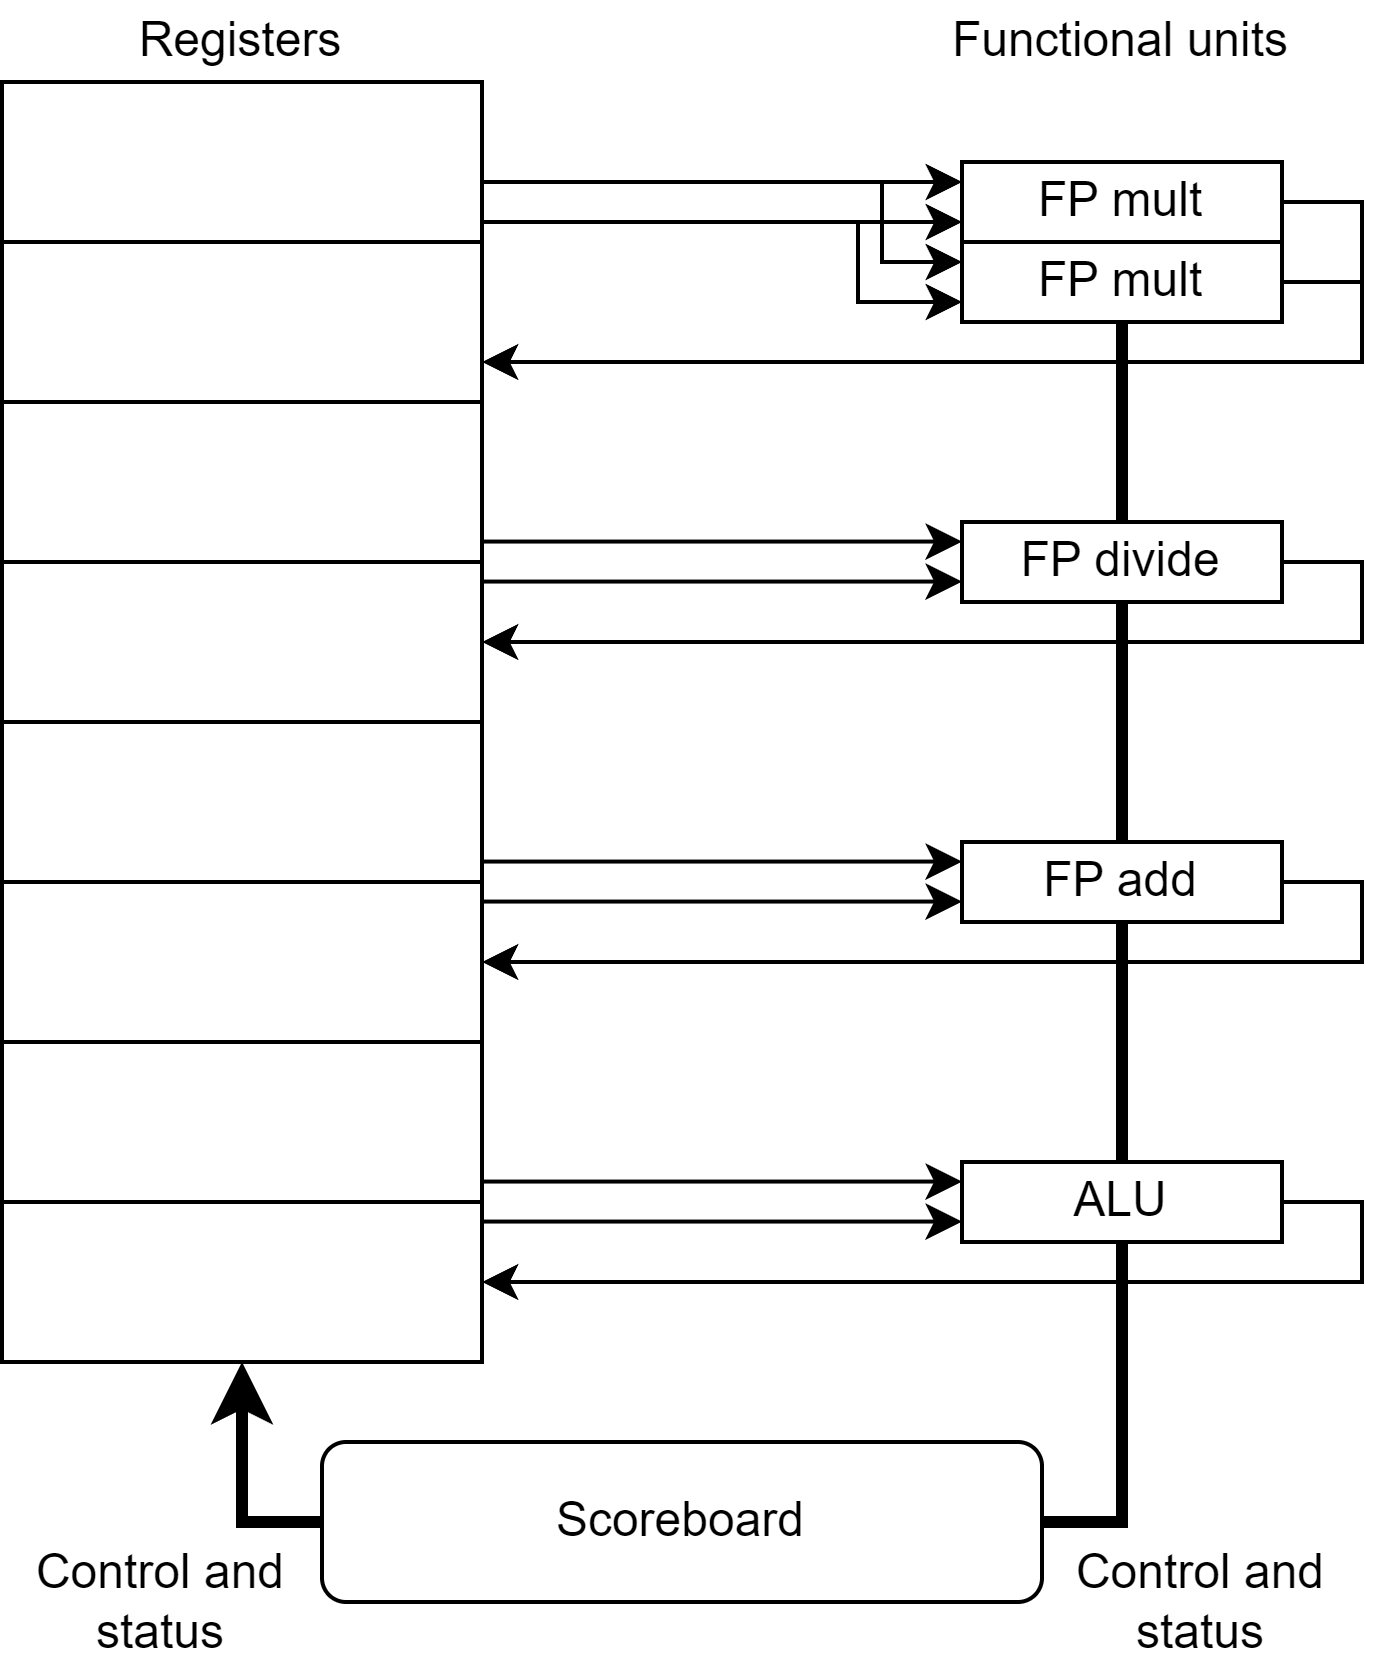
\includegraphics[width=0.5\linewidth]{images/cdc6600.png}
    \caption{CDC6600 scoreboard}
\end{figure}

\paragraph*{Scoreboard operation}
The Scoreboard serves as the hub for hazard management in the new pipeline architecture:
\begin{itemize}
    \item All instructions are routed through the Scoreboard for processing.
    \item It orchestrates the timing for instructions to access their operands and commence execution.
    \item Continuously monitors hardware alterations, facilitating the resolution of stalled instructions for execution.
    \item Governs the timing for instructions to commit their results.
\end{itemize}
This centralized system optimizes performance and ensures efficient instruction flow within the updated pipeline framework.

\paragraph*{Scoreboard scheme}
The ID stage is now bifurcated into two distinct phases:
\begin{enumerate}
    \item Issue: responsible for instruction decoding and structural hazard verification.
    \item Read operands: holds instructions until data hazards are resolved, with an out-of-order execution approach.
\end{enumerate}
While instructions are issued in sequence, the reading of operands occurs out of order.
This innovative approach, facilitated by the Scoreboard, enables the execution of instructions without dependencies, enhancing overall efficiency and throughput.

\paragraph*{Scoreboard control}
The four stages of scoreboard control are: 
\begin{enumerate}
    \item Issue: decoding instructions and detecting structural hazards.
        Instructions are decoded and checked for hazards in program order.
        If the functional unit corresponding to the instruction is available and there is no other active instruction with the same destination register (WAW hazard), the scoreboard dispatches the instruction to the functional unit and updates its internal state.
        If either a structural hazard or a WAW hazard is detected, the instruction issuing process is stalled. 
        No further instructions will be dispatched until these hazards are resolved.
    \item Reading operands: wait until there are no data hazards, then proceed to read operands.
        A source operand is deemed available if no earlier issued active instruction will modify it, or a functional unit is currently writing its value into a register.
        Once the source operands are available, the scoreboard instructs the functional unit to proceed with reading the operands from the registers and commence execution.
        RAW (Read After Write) hazards are dynamically resolved during this stage, enabling instructions to be executed out of order. 
        Note that there is no data forwarding in this model.
    \item Execution: the functional unit initiates operations on the provided operands.
        Upon completion of the operation, it informs the scoreboard about the execution's conclusion.
        Functional Units (FUs) are defined by:
        \begin{itemize}
            \item Latency: the time required to complete one operation effectively.
            \item Initiation interval: the number of cycles necessary to elapse between issuing two operations to the same functional unit.
        \end{itemize}
    \item Write result: upon completion of execution, the scoreboard checks for Write After Read (WAR) hazards. 
        If there are no WAR hazards detected, it proceeds to write the results. 
        However, if a WAR hazard is identified, the instruction is stalled.
        Assuming overlap between issuing instructions and writing results is permitted.
\end{enumerate}

\paragraph*{Implications}
The scoreboard plays a crucial role in managing hazards and dependencies in the instruction pipeline. 
Without register renaming, it must detect Write After Write (WAW) hazards and stall the issuance of new instructions until the conflicting instruction completes execution. 
To accommodate multiple instructions in the execution phase, the system requires either multiple execution units or pipelined execution units. 
The scoreboard maintains the state of operations and tracks dependencies to ensure correct execution sequencing and hazard detection.

\paragraph*{Scoreboard structure}
The structure if the scoreboard is composed by: 
\begin{enumerate}
    \item Instruction status.
    \item Functional unit status: indicates the state of the functional unit (FU):
    \item \begin{itemize}
        \item Busy: indicates whether the unit is busy or not.
        \item Operation (Op): the operation to be performed in the unit (+, -, etc.).
        \item Destination register (Fi).
        \item Source register numbers (Fj, Fk).
        \item Functional units producing source registers (Qj, Qk).
        \item Flags indicating when Fj, Fk are ready (Rj, Rk).
    \end{itemize}
    \item Register result status: indicates which functional unit will write each register. 
        It's left blank if no pending instructions will write that register.
\end{enumerate}

\subsection{Summary}
The key idea behind the Scoreboard is to enable instructions behind a stall to proceed, allowing for the decoding, issuing instructions, and reading operands. This design achieves a speedup of 2.5 compared to no dynamic scheduling. Additionally, a speedup of 1.7 is achieved by reorganizing instructions at the compiler level. However, the benefits are limited by the slow memory (lacking cache) of the CDC 6600.
Limitations of the CDC 6600 scoreboard include:
\begin{itemize}
    \item Lack of forwarding hardware.
    \item Limited to instructions within a basic block, leading to a small window.
    \item A few functional units, particularly in integer and load/store units, leading to structural hazards.
    \item Instructions are not issued on structural hazards.
    \item The scoreboard waits for Write After Read (WAR) hazards.
    \item Measures are taken to prevent Write After Write (WAW) hazards.
\end{itemize}
